\documentclass[notes.tex]{subfiles}

% ---
% Redefinição de comandos para adequar ao formato requerido
% ---
\makeatletter
\renewcommand{\imprimircapa}{

    \DoubleSpacing

    \begin{centering}

        {\bfseries \MakeUppercase{\imprimirinstituicao}\par}
    
        \vspace*{\fill} \vspace*{\fill} \vspace*{\fill} \vspace*{\fill}
        \vspace*{\fill} \vspace*{\fill} \vspace*{\fill}
    
        \bfseries\LARGE\MakeUppercase{\imprimirtitulo}\\
    
        \vspace*{\fill}

        \begin{flushright}
            \bfseries \MakeUppercase{\imprimirautor}
        \end{flushright}   

        \vspace*{\fill} \vspace*{\fill} \vspace*{\fill} \vspace*{\fill}
        \vspace*{\fill} \vspace*{\fill}

        \SingleSpace

        {\bfseries \MakeUppercase{\imprimirlocal} \\ \MakeUppercase{\imprimirdata} }
        \vspace*{\fill}

    \end{centering}
    \pdfbookmark[0]{Capa}{}
    \pagebreak
}
\makeatother

% ---

\makeatletter
\renewcommand{\imprimirfolhaderosto}{

    \SingleSpace
    \begin{centering}

        {\bfseries \MakeUppercase{\imprimirautor}\par}
    
        \vspace*{\fill} \vspace*{\fill}
    
        {\bfseries\LARGE\MakeUppercase{\imprimirtitulo}}\\
    
        \vspace*{\fill}

        \begin{flushright}
            \parbox{0.5\textwidth}{%
                Trabalho de Conclusão de Curso apresentado ao curso de graduação em Ciência da Computação no Centro de Ciências Exatas e Naturais da Universidade Regional de Blumenau como requisito parcial para a obtenção de grau de Bacharel em Ciência da Computação.
            }
        \end{flushright}   

        \begin{flushright}
            \parbox{\textwidth*3/5}{%
                Professor \imprimirorientador, Mestre - Orientador
            }
        \end{flushright}   

        \vspace*{\fill} \vspace*{\fill} \vspace*{\fill}
        \vspace*{\fill} \vspace*{\fill} \vspace*{\fill}

        {\bfseries \MakeUppercase{\imprimirlocal} \\ \MakeUppercase{\imprimirdata} }

    \end{centering}
    \pagebreak
}
\makeatother

% ---

\makeatletter
\newcommand{\imprimirfolhadeassinaturas}{
    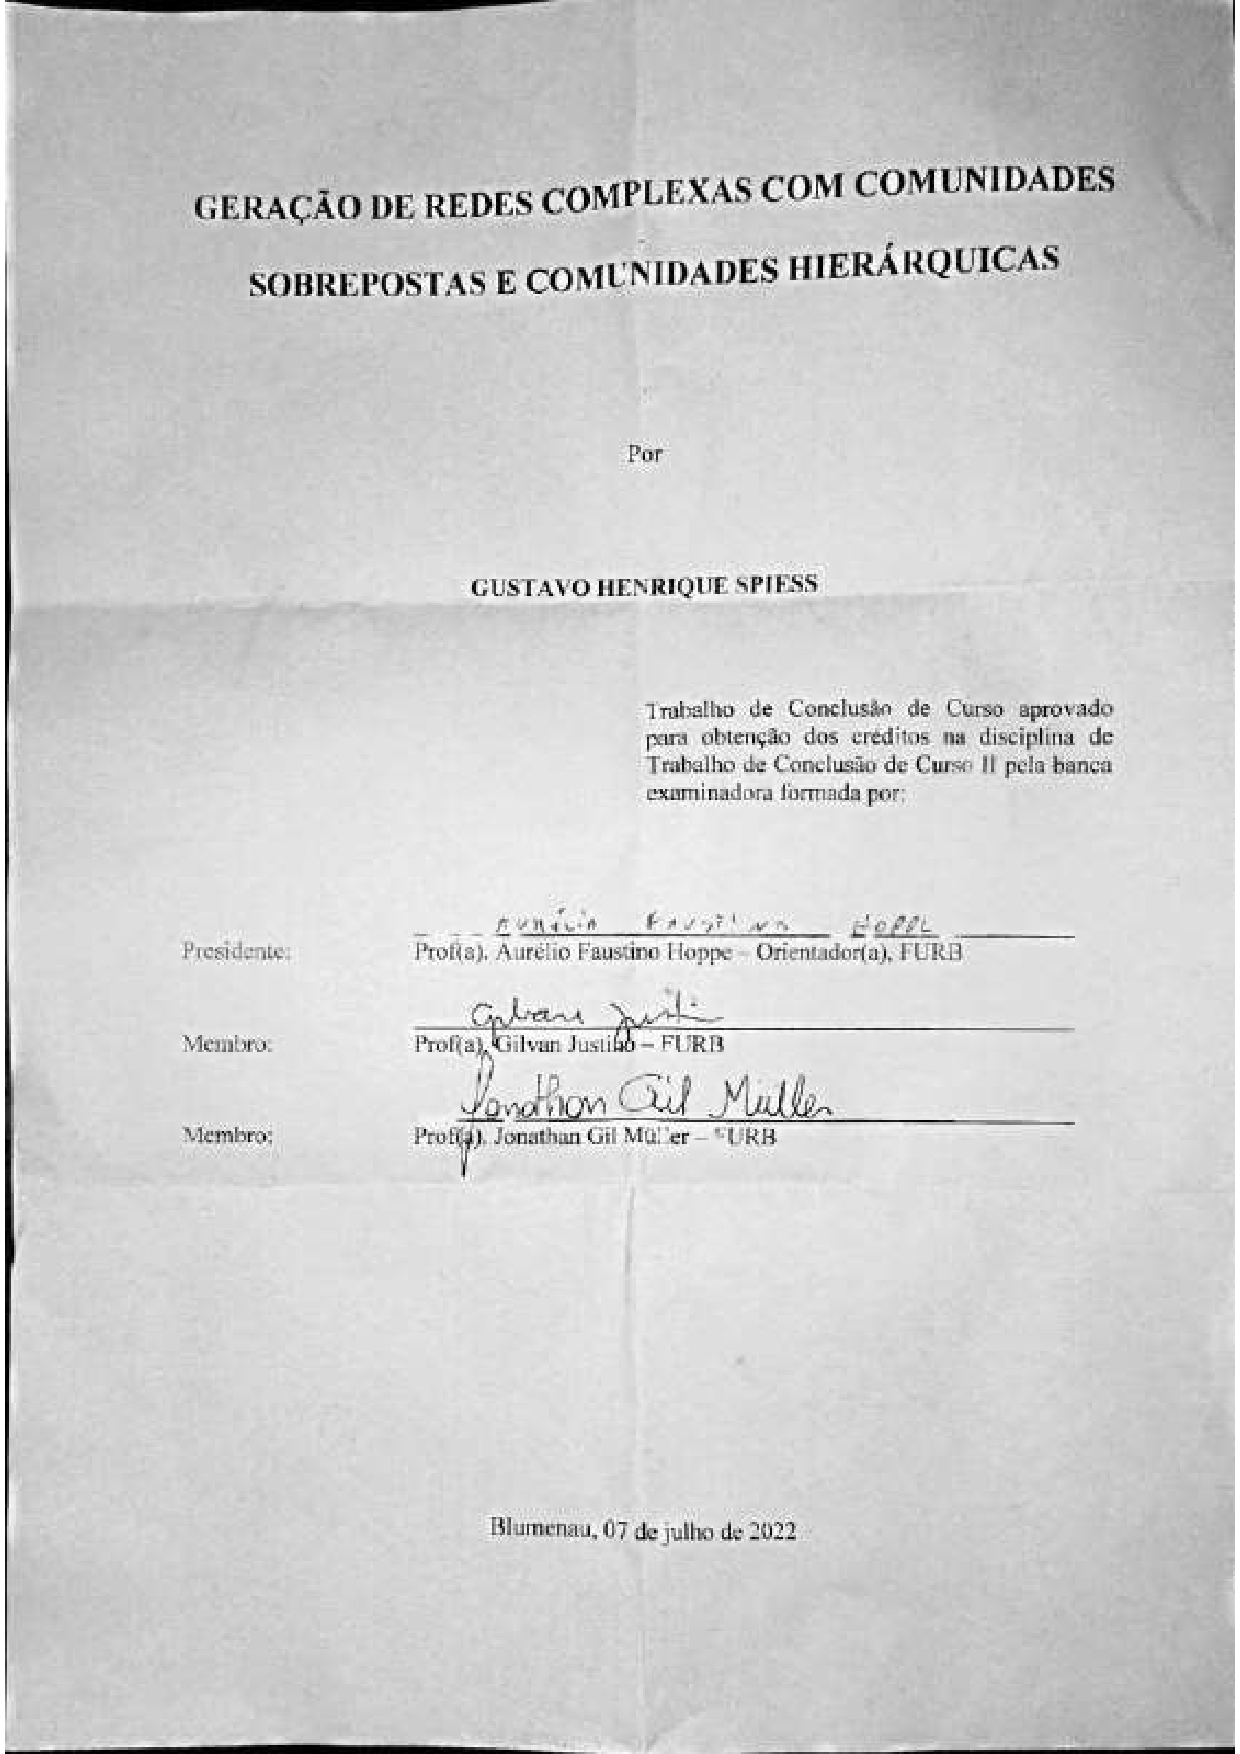
\includepdf{figures/assinaturas.pdf}
}
\makeatother

% ---

\begin{document}
% página de titulo principal (obrigatório)
\imprimircapa

\imprimirfolhaderosto

\imprimirfolhadeassinaturas

\begin{dedicatoria}
    \vspace*{\fill}
    \hfill
    \parbox{0.5\textwidth}{%
        Dedico esse trabalho a minha noiva, cuja paciência em me ouvir falar desse trabalho tornou-o possível.
    }
    \vspace*{\fill}
\end{dedicatoria}
\pagebreak

\DoubleSpacing
\begin{agradecimentos}
    A meu padrinho, Maiko Rafael Spiess, pelo sempre presente incentivo ao estudo.

    Ao meu orientador, Aurélio Faustino Hoppe, por acreditar na conclusão desse trabalho.

    A minha família, por todos os anos de apoio que foram necessários para chegar até aqui.

    Aos amigos que fiz no percurso do bacharelado, pelo apoio recebido.

    Aos professores do Departamento de Sistemas e Computação da Universidade Regional de Blumenau por suas contribuições durante os semestres letivos.
\end{agradecimentos}
\pagebreak

\SingleSpace
\begin{epigrafe}
    \vspace*{\fill}

    \hfill
    \parbox{0.51\textwidth}{%
    ``Se eu vi mais longe, foi por estar sobre ombros de gigantes.''
    }

    \begin{flushright}
    Isaac Newton
    \end{flushright}
    \vspace*{\fill}
\end{epigrafe}

% resumo em português
\DoubleSpacing
\begin{resumoumacoluna}
\bigskip

Sistemas do mundo real são modelados como grafos com atributos, significando uma estrutura de dados onde tem-se uma caracterização dos nodos do sistema, bem como as relações entre eles.
Nesses grafos observados no mundo real, algumas propriedades naturalmente estão presentes na topografia da rede.
Uma dessas propriedades é a tendência de formação de agrupamentos que podem ser descritos como comunidades.
Elas em muitos sistemas possuem a característica de serem organizadas de forma auto semelhantes, isso é, comunidades que são compostas por sub-comunidades, formando uma estrutura aninhada.
Comunidades também tendem, em alguns sistemas do mundo real, a apresentarem áreas de sobreposição, onde nodos pertencem simultaneamente a múltiplas comunidades.
Este trabalho apresenta um modelo algorítmico de geração de redes complexas com comunidades hierarquicamente aninhadas e com comunidades sobrepostas.
O objetivo principal do modelo é a parametrização e controle dessas propriedades durante o processo de construção do grafo para a disponibilização de uma \emph{ground truth} contra a qual algoritmos de detecção de comunidades podem ser avaliados.
A avaliação da presença dessas propriedades é feita utilizando as funções de inércia e modularidade.

 \vspace{\onelineskip}

 \noindent
 \textbf{Palavras-chave}: Redes complexas. Geração de redes complexas. Comunidades. Comunidades sobrepostas. Comunidades hierárquicas.
\end{resumoumacoluna}


% resumo em inglês
\renewcommand{\resumoname}{Abstract}
\begin{resumoumacoluna}
 \begin{otherlanguage*}{english}
\bigskip

It is not rare that real world systems get modeled as attributed graph, meaning a data structure where there is the categorization of the nodes, and also the relationships between nodes.
In this graphs from the real world, some properties naturally happen in the network topography.
One of this properties is the tendency to form clusters that can be described as communities.
In many systems those communities are organized in a self similar way, e.g. communities composed by sub communities, forming a nested structure.
Communities also tend, in some real world systems, to have overlapping regions, where nodes belong to both communities.
This paper presents an algorithmic model for generating complex networks with hierarchical communities and with overlapping communities.
The main goal of this model is the parameterization and control of those properties during the building process of the graph to make available a ground truth against witch detection algorithms can be tested.
The validation of the presence of those properties is done using the inertia and modularity properties.

   \vspace{\onelineskip}

   \noindent
   \textbf{Keywords}: Complex networks. Complex networks generation. Communities. Overlapping communities. Hierarchical communities
 \end{otherlanguage*}
\end{resumoumacoluna}

\pdfbookmark[0]{\listfigurename}{lof}
\listoffigures*
\pagebreak

\pdfbookmark[0]{\listofquadrosname}{loq}
\listofquadros*
\pagebreak

\pdfbookmark[0]{\listtablename}{lot}
\listoftables*
\pagebreak


% \item[IE] -- Internet Explorer
% \item[QE] -- Qternet Explorer
% \end{siglas}
% \pagebreak

\tableofcontents* 

\end{document}
